\documentclass[11pt, oneside]{article}   	% use "amsart" instead of "article" for AMSLaTeX format
\usepackage{geometry}                		% See geometry.pdf to learn the layout options. There are lots.
\geometry{letterpaper}                   		% ... or a4paper or a5paper or ... 
%\geometry{landscape}                		% Activate for rotated page geometry
%\usepackage[parfill]{parskip}    		% Activate to begin paragraphs with an empty line rather than an indent
\usepackage{graphicx}				% Use pdf, png, jpg, or eps§ with pdflatex; use eps in DVI mode
								% TeX will automatically convert eps --> pdf in pdflatex		
\usepackage{amssymb}
\usepackage{hyperref}                             % zelf toegevoegd (via internet gevonden )

\usepackage{tikz}
\usepackage{tikz-uml}
\usepackage{wasysym}          	%eighthnote ~~~ \halfnote ~~~ \twonotes ~~~ \fullnote ~~~ 
	
\usetikzlibrary{fit,positioning}
\usetikzlibrary{mindmap}	
						%\quarternote ~~~ $\natural$ ~~~ $\flat$ ~~~ $\sharp$



\title{Brief Article}
\author{Geert Evens}
\date{}


\pgfdeclarelayer{l1}
\pgfdeclarelayer{l2}
\pgfsetlayers{l1,l2,main}

\makeatletter
\pgfkeys{%
  /tikz/node on layer/.code={
    \gdef\node@@on@layer{%
      \setbox\tikz@tempbox=\hbox\bgroup\pgfonlayer{#1}\unhbox\tikz@tempbox\endpgfonlayer\egroup}
    \aftergroup\node@on@layer
  },
  /tikz/end node on layer/.code={
    \endpgfonlayer\endgroup\endgroup
  }
}

\def\node@on@layer{\aftergroup\node@@on@layer}
\makeatother

\tikzset{
  lvl1/.style={draw,fill=blue!40,rounded corners=1.0cm,inner sep=12pt,node on layer=l1},
  lvl2/.style={draw,fill=blue!20,rounded corners=0.5cm,inner sep=8pt,node on layer=l2},
  lvl3/.style={draw=blue,fill=white,dashed,rounded corners=0.25cm,align=flush center,text width=8em,inner sep=4pt,minimum height=1.5cm},
  title/.style={node font=\LARGE},
  myarrowred/.style={latex-,ultra thick,red!80},
  myarrowgreen/.style={latex-,ultra thick,green!80},
}

\begin{document}

\maketitle{Agile werkdocument}
\tableofcontents
\section{Overview picture}


\tikz \node[rectangle,draw,
label=above:Top,label=below:
Bottom]{my rectangle};


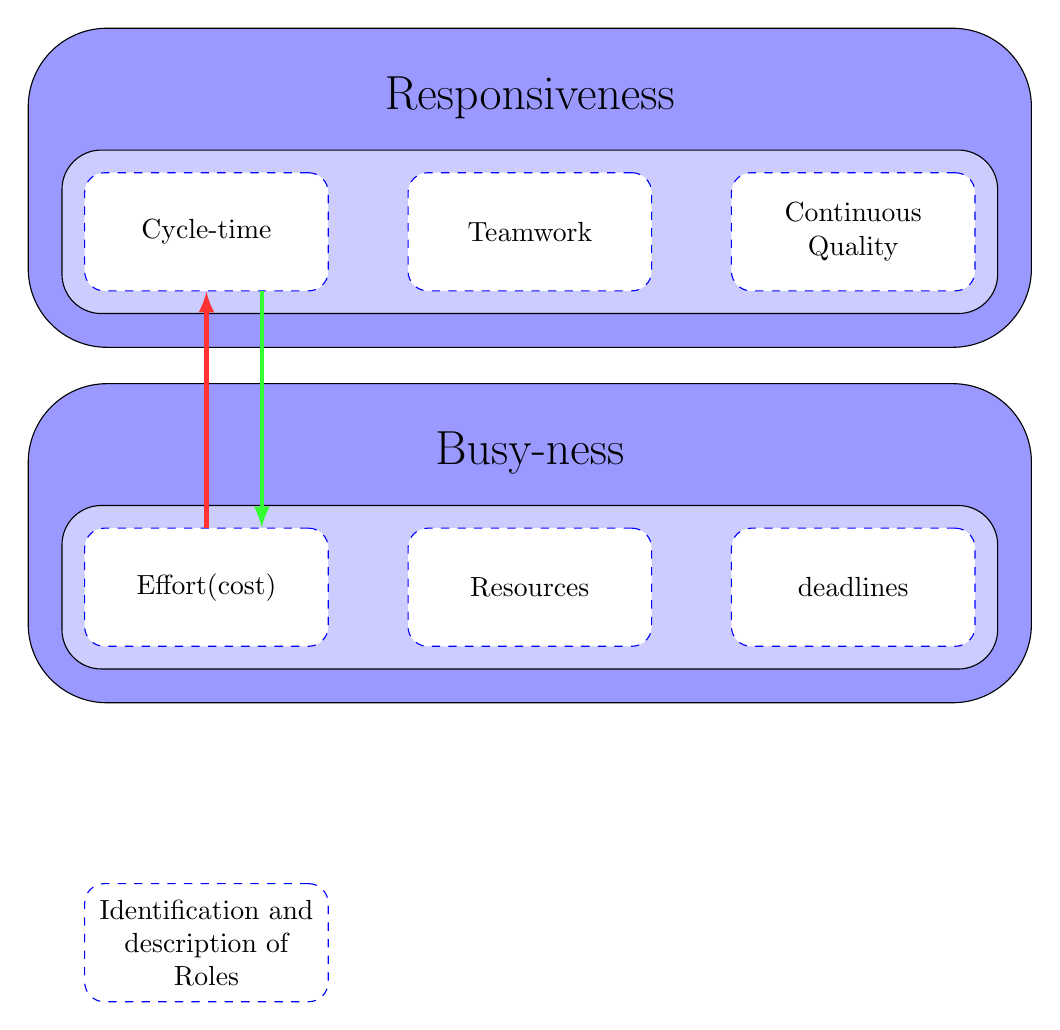
\begin{tikzpicture}
  \node[lvl3] (1) {Cycle-time};
  \node[lvl3,right=of 1] (2) {Teamwork}; 
  \node[lvl3,right=of 2] (3) {Continuous Quality}; 
  \node[lvl3,below=3cm of 1] (4) {Effort(cost)};
  \node[lvl3,right=of 4] (5) {Resources};
  \node[lvl3,right=of 5] (6) {deadlines};
  \node[lvl2,fit=(1) (2) (3)] (group1) {};
  \node[lvl2,fit=(4) (5) (6)] (group2) {};
  \node[title,above=0.2cm of group1] (title1) {Responsiveness};
  \node[title,above=0.2cm of group2] (title2) {Busy-ness};
  \node[lvl1,fit=(title1) (group1)] (group1lvl1) {};
  \node[lvl1, fit=(title2) (group2)] {};
  \node[lvl3,below=3cm of 4] (roleID) {Identification and description of Roles};
  \draw[myarrowred](1.south)--(4.north);
  \draw[myarrowgreen] ([xshift=20pt] 4.north)--([xshift=20pt] 1.south);
\end{tikzpicture}


\section{Our intuition fools us}
Humans have known biases.

\section{Matrix intuition fooling us}
\subsection{Focus on efficiency makes the system slow}
\subsection{task based management can destroy passion}
\subsection{Milestones result in pressure quality decrease}
\subsection{Slow system, passion destruction and quality decrease enforce each other}

\section{Long term positive agile effect}
\subsection{Reduce leadtime makes the system more responsive and efficient}
\subsection{Working together in team gives room for passion and talents}
\subsection{Proactive quality improvements makes software more predictable}
\subsection{Passion, responsive system and high quality software enforce each other}

\section{Technology versus organization structures}
\subsection{High cohesion - low coupling}
\subsection{Power of visuals}

\section{Matrix versus agile}
\begin{tabular}{ l l } in the system & on the system  \\ direct & indirect  \\ concrete plan & clear direction \\ things right & right things \\ failure avoidance & failure recovery \end{tabular}

\section{Scrum as goal}
Scrum is nice set of practices , not a goal itself. Do not agree. Scrum forces you to invest on the right things. 
Agile mindset is a long term investment driving us to do right things for productivity for productivity
Why now possible  , measureable

\section{Oneliners}
\begin{itemize}
\item Scrum is a bouned environment for action (gunther Verheyen)
\item Als je open bent over je sterktes en je zwaktes dan kun je dingen doen die bij je passen (Hans Duisters)
\item Busy-ness creates more busy-ness
\item Eerst het plaatje, dan het praatje
\item Take less to get more done
\item Command and control creates followers. 
\item we hebben 2 oren en 1 mond. Gebruik dat dan ook in deze verhouding.
\item scrum breaks the rules. It is even designed to do that. \\
\end{itemize}
 
\section{statements}
\begin{itemize}
\item beste protector van het team is het team zelf.
\item main cost is NOT delivering value.
\item busy-ness creates more busy-ness. 
\item Only happy people will make great software
\item Failure recovery is more important than failure avoidance. (denk aan kinderen die maar proberen).
\item the organisation is not a machine. But an organism, a set of human interactions - the system is not the sum of it?s parts. It is the product of the interactions
\item Have trust that people do right things.
\item Je bent een manager van jezelf. 
\item Als je geen plannen maakt voor jezelf wordt je ingezet in andermans plannen.
\item Je moet niet harder werken, maar slimmer werken
\item Productiviteit is omgekeerd evenredig met complexiteit. \\
\item Kracht van productiviteit zit in eenvoud en samenwerken, niet in complexiteit en het harde spel (concurreren).
\item zeggen wat je doet en doen wat je zegt. (=pro-actief communiceren en ... Je moetgeen dingen toezeggen (beloven) die nog niet van jou zijn.)
\item Didier: The proof of the pudding is in the eating.
\item Niet grote bazen maar grote ideeen veranderen de wereld. \\
\item People forget what you say and what you do, but they'll never forget how you make them feel. \\
\item We hebben een hekel aan sleur, maar zijn bang voor verandering
\end{itemize}
 
 
 
\section{mindmap from principles to practices}
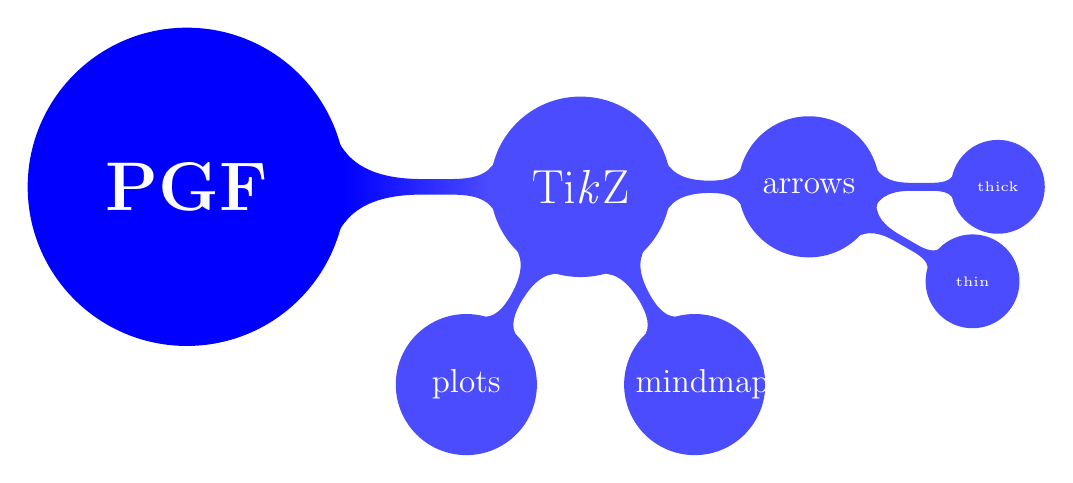
\begin{tikzpicture}
  \path[mindmap,concept color=blue,text=white,
    level 1 concept/.append style=
      {every child/.style={concept color=blue!70},sibling angle=-30}]
      node[concept] {\Huge\bfseries PGF}[clockwise from=0]
        child {node[concept]{\LARGE Ti\emph{k}Z}
            child{node[concept] {\large arrows}
                child {node[concept] {thick}}
                child {node[concept] {thin}}}
            child{node[concept] {\large mindmap}}
            child{node[concept] {\large plots}} };
\end{tikzpicture}

\section{Tips}
Durf veren in je kont te steken
Management meenemen, transparant, in kleine stappen.

\section{Boekentips}
Reinventing organisations , laloux

\section{externe bedrijven}
Cegeka, cipal, zappware

\subsection{prowareness}
Goed prowareness : 
\begin{itemize}
\item open over salarissen
\item Geen old fashioned job interviews : minder op wat. 
\item Samenwerken : focus hierop.
\end{itemize}

\subsection{coolblue}
work hard play hard, documentaire op youtube


\section{audiobooks}
Not every measurement counts. Not everything that counts in measureable

Op 31-mei-2015, om 21:36 heeft Geert Evens <evensgeert@gmail.com> het volgende geschreven:

20 30 \% meer tijd. anticipeer. Laat weg \\
Kernactig afsluiten : verwijzing begin.\\
Managen jezelf : voornemen alleen is niet genoeg.  moeten gedrag sturen \\
bewust gepland versus onbewust ongepland \\
nut - andere mensen - controle. \\
automatische goed/niet goed. \\
95\% op automatische piloot. \\
jukebox speler \\
beloningen of straffen worden direct geinterpreteerd. \\
durfen : doelgericht belonen. \\
Wanneer waren de uitzonderlijke momenten. \\
Hoe kan ik zo zijn zoals ik ben op mijn beste momenten. \\
Overtuigingen zijn een beeld van de waarheid. \\

Prikkels = conditionering. \\
Mensen hebben hekel aan verliezen, niet aan veranderen.\\
Doel en gedrag zo concreet mogelijk maken. \\
Gedrag meetbaar actief en persoonlijk.\\
vermijden van crisissituaties kan in begin, maar uiteindelijk toch nodig.\\
beloningen moeten echt voldoende zijn.\\
leren bij volwassenen gaat zelfde als bij kinderen.\\

geheugensteuntjes, beloning, countering.\\
directe feedback : meten en belonen.\\

Lichaamstaal : \\
naam noemen, positief in leven staan. \\
Woord nemen : noem de naam.  \\
oogcontact maken ook belangrijk. Hoffelijkheid. \\




\section{Todo} 
every has a plan until he is punched in the face : tyson. \\
Succesvolle startups : timing was most important. team is 2nd \\

Een team stuwt je vooruit \\
di�ten maakt dikker (knack juni) : focus op resultaat werkt averechts, focus op omgeving is veel blijvender en duurzamer. \\
Covey circle of influence : beinvloed de omgeving om echt groei te realiseren. \\

reasons why:
\begin{itemize}
\item Because focus on efficient management makes the system slow.
\item Because task based management can destroy passion for the job.
\item Because Self organizing teams bring innovation is a fast changing environment.
\item Because a responsive system is key for real flexibility.
\item Because real grow occurs indirect.
\end{itemize}

\section{DP ASML Sioux}
Begrijp dat sommigen productiviteit laag vinden. Mijn motivatie is ook nooit zo laag geweest en heb me nooit zo als een speelbal gevoeld.


\section{annekdotes or stories}
Molenaar - mensen met tractor hebben geen tijd.
helpdesks : efficient?

\section{Beeldspraak}
Rode lichten versus ronde punten.eml> \\
blue black or white gold dress ? \\
Out of box denken : koeien blijven binnen de lijnen ook als geen echte roosters zijn. \\
alice in wonderland : gaat een wereld open.\\
Hout nodig -> ga hout halen. Was voor boot, dus verkeerd hout, ? . Specifieer waar je het hout voor nodig hebt !\\
Koeien en lijnen op de weg\\

\section{extern resources}
db - infoq is interessante resource.eml> \\
<db - A3 thinker's action deck.eml> \\

\section{definitions}
Culture : Stuff that people do without noticing it. \\
PDD development : pain driven development \\

 \section {dagboek}
 
 \subsection{augustus}
different models for different responsibilities versus not good for maintenance / much overhead ? \\
Albert van der werf : gras altijd groener wel 3x gezegd => erg afwachtende houding. bij hem ook geen go ivm jenkins server \\
Mijn leuze nu : productivity is about simplicity and cooperation.\\
 
 \subsection{juli}
 Eigen idee : productiviteit is durven investeren en dan loslaten
 Op radio, lingery vandevelde.
\begin{itemize}
\item Evaluatie moet continue process zijn. Geen administratieve rompslomp.
\item Bedrijf moet bezig zijn met klanten, met energie van de mensen, passie.
\item Het mag niet zo zijn dat je maanden moet wachten op dat moment.
\end{itemize}

reinventing organizations, Laloux

 
\subsection{juni}
%\url{http://www.nytimes.com/interactive/2015/02/28/science/white-or-blue-dress.html?_r=0}

 
Waardering zal je niet krijgen : Weggaan met beleid. \\
Word gecontacteerd door Luis om iets over Scrum te vertellen. \\
DP pionierswerk:\\
Continuous integration \\ 
Teamwork -> bord, pull system, GIT\\
TDD, unittests ,
Coverage metingen
scrum, assemblies : zelfde stramien - past niet: eerst zorgen dat het past, en dan pas toepassen. \\

it is not that you are doing the right thing if someone says so.\\

Idee : agile in lego.

 Jupiler league, championsleague, winnaar championsleague. Waar willen we spelen ?

��         Programmeren kan iedereen. Software engineering is iets anders \\
�         Fit for future idee : aangegeven in kaart brengen van doorlooptijden.\\
�         Enige constante in heel de miserie is GL/PL\
�         Tot nog toe sprong ik steeds in een gat. Nu is er geen gat. Blijf wat op mijn honger zitten. Weinig uitdaging.\\
�         Als verstoringen weg zijn gaat het opeens veel beter?\\
�         Zoveel winst te halen in team ? kwaliteit ? flexibiliteit. Dat moet je door de mensen zelf laten doen.\\
�         Dingen laten delegeren en obstacles wegnemen bij personen : testtijd dag later en lijstje Freek verkorten: succesvolle acties\\
�         Dingen worden rechtsstreeks bij Edwin aangekaart. Betrokkenheid van het team hierover als vragen komen erg laag. Mijn invloed is erg laag. Ik werk in een andere rol.\\
�         Podcast : naar achter lopen in standup: mensen moeten naar elkaar vertellen.\\
�         Podcast : self-destructing teams: iemand als baas zien en dus problemen doorgeven.\\
�         Productief bedrijf investeert in 2 dingen : gouden eieren en welzijn van de gans.\\
�         Gunther Verheyen : Wie is hier manager ? => manager van je eigen leven. >>\\
�         Heel erg sceptisch -> voorzichtig zijn met dingen aan te passen\\
�         Kloof tussen management en werkvolk is nadrukkelijk aanwezig. Weinig betrokkenheid.\\\\
�         Overdreven met complimenten gegooid -> werkt motiverend voor de kinderen. Willen het echt goed doen\\
�         Precies alsof grootste kind alle speelgoed van de kleinste op de grond gooit en dan roept dat die het moet opruimen omdat het van haar is.\\
�         Er zijn er 3 die zich met het proces bezig houden. \\
�         Gevoel van 5de wiel aan de wagen. Edwin en Freek doen nu alle voorbereiding en zit niet veel in voor mij op dit moment.\\
�         Krijg hier nu wel het ivoren toren gevoel. Veel voorbesproken tussen Freek en Edwin. \\
�         Amanda Palmer : take all the pain and wear it as a shirt.\\
�         Leuk, ik heb bijna de meeste registraties voor mijn presentatie.\\
�         Ik moet issues was sneller dingen vlaggen en zien en met mensen praten.\\
�         Support met Pieter Custers een hebben over overzichten maken.\\
�         Support moeten we iets mee doen. -> beter overzicht wat voor issues en mogelijke verbeteracties.\\
�         Freek: High level plan statisch. Ik vind dynamisch.\\
�         Planning meeting : ging erg rommelig en prioriteit en voorbereiding was dan toch niet in orde.\\
�         Complexity los je niet op met complexity.\\
�         Agile, my why\\
�         Support slorpt toch wel wat tijd op.\\
�         Enige constante bij alles wat misgaat is PL en GL. Heel team veranderd op jaar tijd.\\
�         Fouad komt binnen en ontgoocheld dat niks ?echt? gedaan is.\\\\
�         5jarige kindjes kunnen hun kleren nog niet goed aandoen, ?\\
�         Verbaasd dat zelfs Sioux niet agile doet.\\
�         Toch nog direct taken geven aan team members.\\
�         Frustratie en ongeloof toch diep bij Freek ook.\\
�         http://www.targetprocess.com/articles/speed-in-software-development.html\\
�          

 \subsection{Januari/februari}
Niet de bedoeling scrum te verkondigen ! -> blokkeert ruimte\\
Agile is over voedingsbodem, over investeringen, over lange termijn visie.
Zit te denken om iets met voedingsbodem te doen. 
Serdar zit er negatief in. Niet zijn droomjob. Michel neemt het risico.
Agile aanvaard bij engineers, top level managers, middle management is issue.
Waarom kreunt een hollander als hij klaarkomt. Omdat uit eigen zak moet komen.
Neen is ook een antwoord \\
Vertrouwen is het kernwoord. Is er dus niet. \\
Jeroen zit overal op de rode draad. Kan niet verder. Te bespreken in sprint start. Opties overlopen die we hebben.\\
Grote bezorgdheid over de kennis die verdwijnt bij DP. En Tom gaat ook vertrekken. Kan je de vraag stellen waarom.\\
Het halen van sprint doelen begint bij het halen van dagdoelen. Focus draait rond het zetten en halen van doelen.\\
Ik ga geloof lange termijn investeringen, alhoewel ze niet logisch lijken.\\
Filters proberen te mappen op stakeholders\\
Tester onzeker over FFM testen. Geen respons om te testen.\\
Geen backlog voor Pieter. Hoe dit fixen ? \\
Agile control loop versus traditional control loop \\
Rini : Agile = kwaliteit van het begin, niet op het einde.\\ 
About.me page misschien nog iets. Gezien bij Ben Linders. \\
Routine en visueel maken. Zo ook bij Reggy gezien. \\
Afrekencultuur: en dan kijkt men nog eens in de ogen om commitment te krijgen.\\
Safe training iets voor mij ?\\
Van process gestuurd naar mens gericht. \\
Didier had zelf al 15 manweken opgeschreven voor een eenvoudige sync. Ik zou zeggen 18 manweken.\\
Ik geloof in een zelf sturend team. Samen aan werken.\\
Challenge, mastery and making contribution : why people do things for free.\\
\textbf{Management is ok if you want compliance. If you want engagement, self-direction is better (Dan Pink).}
Idee : voice van team in sectie van nieuwsbrief ?\\
Helemaal overtuigd van scrum, alleen weg er naartoe moet anders.\\
Linkedin groepen bekijken tussendoor. Pulse applicatie met tegels\\
Scrum steering comitee. Frameworks LESS en SAF(V?)E. Prowareness deployt SAFE ? \\
Samen werken belangrijk. Maar hoe meten ? KPI?s ?\\
Prowareness kwam ter sprake.\\
Niet ter sprake: maar meeting meer gebruiken om elkaar te helpen ?\\
Volgens mij investeren in juiste backlog op orde. Gaat helpen. Epics en versions.\\
Freek ziet geen voordeel om met meer dan 2 aan 1 epic te werken. Dan kunnen we minder in parallel doen.\\
Linux testen blijken niet te werken. -> devpatch creatie gaat fout.\\
Didier met oogpunt patch erdoor te krijgen. Raoul echt op kwaliteit en processen.\\
Sogety gaat twist doen. Meeste en vervelendste werk is waar systeemkennis voor nodig is. Welke recipes, welke configuratie: uitzoeken en organisatie ingaan om met mensen te praten. Dit wordt moeilijker.\\


\subsection{Mei :}

\subsection{April :}
Phenospex : iets met biotechnologie ?\\
speak with right intention, not attention.\\

\subsection{Maart}
Voel je krachtiger in 10 min : link\\
Scrum wordt gedoogd, niet geaccepteerd.\\
Management is too important to leave it to managers\\
Treating Humans Like People\\

\subsection{Januari}
Edwin van der velden slorpt toch wat tijd op. en vraag om echt tijd te meten. Controle based. \\
Om je dromen waar te maken, moet je wakker zijn. \\
Denk nog eens aan fishbowl oefening. \\
to reach goals, don?t focus on goals but on behaviour. \\
Mike Richardson - agility gap. (between demand and supply). gap increases. Overwhelmed. Integration happiness, success. \\
Productiviteit niet op controle en consensus, maar op kwaliteit, mensen en doorlooptijd. -> vereenvoudig ! \\
Consensus model blokkeert. Meer structuur blokkeert. Hakken in het zand. \\
Meer hokjesdenken -> meer eigenbelang, minder gezamenlijk(ASML) belang. \\
In combinatie met consensus model verschrikkelijk verstarrend. \\
Evoluties nu richting devops, meer samenwerken, betrekken, minder tegenwerken \\
Wordt niet op juiste bottleneck geinvesteerd. Niet competence maar tevredenheid, doorlooptijd en kwaliteit moet geinvesteerd worden. : ASML focuses on the wrong priorities \\
Stopzinnen voor moeilijke mensen :
\begin{itemize}
\item Spijtig dat je er zo over denkt."
\item ?Dat is jouw mening.?
\item ?Misschien heb je gelijk.?
\end{itemize}

Minister van vereenvoudiging in Belgie : goede zaak want vanzelf gaat het niet.\\
Men veegt voor eigen deur maar gooit het vuil bij de buren.\\
Men moet geen muren bouwen rond mensen maar juist de muren slopen.\\
Belgisch wegdek : vermijden dat 2x zelfde fout. Maar op een gegeven moment valt er niet meer over te rijden. Investeren in het vermijden van ongevallen is beter.\\
Echte probleem erkennen is productiviteit/efficiency. En dat krijg je niet beter door hardere spellen te gaan spelen. Werkt concurrerend gedrag in de hand ipv meer te gaan samenwerken.\\
Component ownership in 20\% -> werkt niet. Krijg geen respons van mensen.\\
Structuur niet haaks op de business zetten. \\

Idee duikt toch weer op om vanuit spreadsheet een site te maken. \\
Raoul en Didier gesproken : Sioux trekt gat en zadelt ASML op met een probleem. \\
Is nog geen oplossing voor. Geen nieuw werk en niet onnodig lang ophouden. \\
Onderhandelingsruimte: Expertise in systeemtest fase. \\
Zo snel mogelijk de bom laten barsten. Risico vermijden. \\
Linne drumt wel echt graag? misschien iets mee doen. \\
Voordeur/achterdeur verhaal werkt wel aan koffiemachine.  \\

Kracht zit in de samenwerking, maar dat is niet te vatten in een spreadsheet. \\
Hoog in toren deadline geroepen, dan SP vastgepind, laatste redmiddel mensen bijzetten. Helpt niet. Steeds zelfde verhaal.\\
Meeting met DP team gehad : hele GIT gebeuren gaat wel meer en meer op clearcase lijken, met mensen die op knoppen moeten duwen en approvals moeten geven.\\
Jeroen vroeg waar ik was. Geeft goed gevoel dat team ernaar vraagt\\
Nog geen nieuws over mijn vervanger.\\

\subsection{December}
Kwaliteit, samenwerken, vereenvoudiging -> voordeur activiteiten. Beperken de kans op fouten. Gaan over beleid en worden onderschat.\\
LO autotester is a drama. Clean en zo doet het niet zoals verwacht.\\
Mentaliteitswitch. Meeste stoort de mentaliteit om oorzaken bij mensen te zoeken. Vertrouwen dat iedereen het beste voor heeft doet al veel.\\
Autotesters die semi automatisch werken : OTED met opties.\\
Frustraties maskeren de echte problemen. Blaming ed, extra mgmt laag verhoogt overhead, maar is niet de grond van de zaak.\\
Stefan Steenvoorden : flatline bij integratie bij hen. Zelfde dus als intern.\\
Even aankijken : vervanging is er voor mij en overdracht zou mogelijk moeten zijn.\\
16/12 met Florin gepraat over plannen. Ik zou plan maken.\\
Je moet een kip niet als een eend behandelen en in het water gooien.\\
Scrum, autotesters, etc zijn geen doel op zich. Wel nuttig.\\
Beste stuurlui staan aan wal : Wat ASML groot heeft gemaakt speelt het ook parten nu.\\
Kritiek op personen\\
Verliezen tijd door UT/Cov/? Tijd winnen -> Hypotheek op kwaliteit -> spiraal\\
Micromanagement -> controleren : concurreren ipv samenwerken. Communicatielijnen niet aanwezig -> roddelcircuit.\\
Ik krijg heel goed feedback van collega?s, vooral lange termijn visie.\\
Plan afspreken met Florin : uitfazering + concreet plan delivery.\\
QBL sync is pas mogelijk nadat datpath migration opgeleverd heeft. Dit zorgt voor vervelende vertraging voor dose CSR.\\
Arthur heeft over communicatie : We zijn gaan communiceren ! dat hielp om een gekende fout die bij de klant de kop op stak naar boven te krijgen.\\
Martijn presentatie om communicatie naar voren te halen, richting SP1 -> positief \\
Volgende datums begin development finish development end beta test : 
5579    10/15/2013       5/13/2014       2014-03-02 (2014-08-28) \\
Kritisch zijn ten opzichte van samenwerken. Rene slaat hier nagels met de kop. We zijn doorgeschoten betreft kritisch zijn. Mag niet ten koste gaan van samenwerken. \\
Omgeving hebben waar echt verbetering getolereerd wordt en continuous integration aangemoedigd wordt.\\
Echt zonde dat ASML helemaal links blijft zitten.\\
Team uitbouwen wil ik in mijn job description hebben zitten.\\
Samen iets van maken betekent samenwerken.\\
Ik ben vertrouwen in ASML management een beetje kwijt. GL zit een beetje gesandwicht. \\
Eilandvorming, controle => daar moeten we nu juist vanaf. We staan nu met zijn allen in de file \\
Nieuwelingen net van school raken gedemotiveerd, planningen zijn nu al onhaalbaar. Maar wordt gewoon doorgecommuniceerd. \\
Ik sta verbaast dat zo naar competence based gestuurd wordt. Op lange termijn wekt dit frustratie op aan requirements en timing verwachtingen. \\
Ik wil echt iets uitbouwen en/of creatief zijn. Productiefste team was DP team. \\
Goldplating daar is ASML nog heel ver vanaf. \\
OTED autotester behoorlijk spinnenweb maar behoorlijke testen \\
Toch eens voorstellen om het runnen van de LO autotester te vergemakkelijken. \\
Echte groei is steeds indirect: zie ook kanban dat stuurt op leadtime, niet op effort. Presentatie Mark Bruls. \\
Echte ervaren mensen zitten niet meer mee in het team. \\
MPS lijkt heel leuk om te doen. Hier web content mee genereren lijkt erg leuk. \\
Er loopt heel wat te gebeuren. Mogelijk gaat Raoul toch nog dwarsliggen? \\
Focus op autotester \\

\subsection{November}
Via Michel begrepen dat er terug twijfel was bij mij als scrum master. Mogelijk nadat hij Raoul gebeld had ? \\
Ervaringen presentatie: \\
Had meer mogen kijken op het blad. Het vanbuiten kennen viel tegen \\
Wel goede medewerking van collega?s. \\
Had niks om mee te geven na de presentatie. \\
Mooi dat Mark mij gevraagd heb omdat ik regelmatig iets post over agile. \\
Verwachting ASML meer een service bedrijf. \\
Poging nu: invloeden in kaart brengen. \\
Prioriteit gesteld en Temo gaan helpen \\
Plan/done lijstje bijhouden werkt goed. \\
HET LEVEN IS ALS EEN SPIEGEL, JE KRIJGT HET BESTE RESULTAAT ALS JE LACHT ! \\
Aan koffiemachine: men weet niet wat Ad 3 weken lang gedaan heeft -> strakker plannen ??? \\
Wienand Drenth is de SIA schrijver voor Imaging optimizer 2. \\
Meegaan in de cliches en er een schepje bovenop doen werkt qua humor. Bv ik heb herhaling nodig voor iets gebeurt (man-vrouw relatie). \\
Requirement tooling nodig ? => vrijheid om creatief te zijn ontbreekt. Angst voor verandering. \\
Jeroen Leenders: leuke sketch over Belgische regeringen. \\
Wat is dat toch met Sioux. Waarom gaat iedereen weg ? \\
Wij zij denken: wij worden deel van probleem. Polarisering \\
jason fried: real problem are m\&m?s, managers and meetings. \\
Yves Morieux: blame is not for failure, only for failing to helping or fail asking for help (ceo lego). \\
it?s all about the people centric, quality driven, feedback oriented \\
Echte groei is steeds indirect \\
Scrum master tries to keep the engine run smoothly \\
Omdat we mensen zijn : focus ligt op mensen niet resources. abstractie die veel wegmodeleert. \\
Slechte staat van de weg : Ofwel oplappen nadat problemen er zijn ofwel vermijden dat er iets zal gebeuren : Vereenvoudig met hoge kwaliteit, zowel op management als software vlak. \\


\subsection {November}

blog : bekijkheteensanders ?? Persoonlijke interesse. \\
ted.com : Tali Sharot: The optimism bias. \\
need positivism\\
Dan Pink : against incentives, blocks creativity, candle problem. Mismatch what business does and science knows. Extrinsic motivators do harm. Get money from the table. rudimetary \\
skill -> higher reward, worse performance.\\
Shawn Achor \\
Ken robinson Ken Robinson: How schools kill creativity. If you are not prepared to be wrong you will never be creative. We grow out of creativity.\\
Brene brown : The power of vulnerability.\\
Dan Ariely\\
Hans Rosling : The best stats\\


https://twitter.com/favorites   : Af en toe bekijken.\\
Stel moment van rondsurfen uit tot na de standup. Werkt goed.\\
Wat ligt afwerken ging prima. Kleine dingen volledig afwerken.\\
Tracy helpen door bij mensen te informeren (Erik) heeft geholpen en geapprecieerd.\\
expliciet vraag gekregen waarom ik niet veel klaag. Ik heb geantwoord dat ik acceptatie faze zit. Had meer moeten zeggen dat ik juist vind dat het hier allemaal prima gaat (ironisch). -> meegaan.\\
Zelf naar arch vragen of duidelijk was ging goed (offset bepaling) -> positief antwoord.\\
Arch weinig proactief over de vloer. Ivoren toren principe. Jammer.\\
clean desk voelt goed. Documenten digitaal maar goed overzicht.\\
Samenwerking Tracy goed. Zij ook dingen uitgezocht/geprobeerd.\\
Documenten digitaal -> werkt goed.\\
Michel : Drive zit erin. Goed om te horen.\\
Fouad gesproken 7/11  => let op gebruik van metaforen.\\
Team heel positief dat ik rol zou spelen\\
Hij ziet zichzelf als een hamburger en heeft zelf ook moeilijk gehad.\\\\
Zelf voordeur geintroduceerd.\\
idee van sprint labels gelanceerd -> focus en flexibiliteit.\\
Vertrouwen komt te voet en gaat te paard.\\
Routine is belangrijk -> plan retrospectives en demo?s in.\\
Zorg toch steeds dat je bij commitments factor 2 in rekening brengt.\\
Dag ervoor alvast inplannen werkt goed.\\
Heel vroeg in de morgen weer concreet inplannen -> werkt ook goed.\\
Dagboek iedere morgen bijvullen \\
Frank van Morselt eens polsen voor samenwerkingsverbanden.\\
Lijst van scrummasters moet ik toch eens gaan opzoeken\\
Nick verkeerd gebruik CS gewezen. -> goed! -> communicatie\\
Stef. Weinig frisse wind. Hogere posities: weinig extern gezien. Kruisbestuiving te weinig.\\
Planning meeting gedaan zonder Vincent/Stefan => nabespreking bij standup.\\
Eindig de dag eens met een evaluatie en planning van de volgende dag.\\
Probeer een tip :http://www.opencircles.nl/blog/productiviteit-tips\\
Performance probleem andere project : blame DK -> productief ?\\

\subsection{Oktober}
Stefan soortgelijke discussie over efficiency met Raoul.\\
Mijn idee: dingen uit reactie gedaan -> controleren,op de huid zitten-> contra-prod\\
asml heeft echt een probleem ! Wachten tot laatste moment en dan escaleren is de way of work. Wordt zelfs geaccepteerd.\\
Roepen wat fout gaat en anders moet is anders dan de oplossing. En de oplossing is niet micromanagement, en ook geen muren rond mensen en ook niet documentatie.\\
Gesprek met Michel:\\
tester in het team, kwaliteit is ruimte voor, Fouad, Freek -> gelijkaardige visie. Verder opzetten wat ik/wij hadden opgebouwd.\\
arch hamert op realistische schattingen. Zeker haalbaar. Gewoon copy replace. Hangt af van de kwalificatie. Direct al probleem met grant en niet kunnen uitchecken.\\
Architect communiceert dat ik eerste voorstel moet uitwerken. En verzwijgt 2de voorstel. Terwijl achteraf bleek dat het 2de voorstel hetgeen is waar iedereen achter staat. Gaat in tegen open communicatie\\
Eerste voorstel op papier : direct reactie dat niet volledig is, etc. Was niet de bedoeling! Zijn er toch uitgeraakt ?! Hij doet verder communicatie naar Dimitri.\\
Presentatie ideeen doorgemaild. 25 november ben ik aan de beurt.\\
Idee : Agile brainstorm. Groep die mag groeien. - Groep-discussies.\\
Gesprek met Stefan :\\
Niet met uren werken, maar met briefjes\\
Backlog grooming iedere week\\
Heb bezorgdheid geuit dat communicatie met architect beter loopt -> we gaan grooming introduceren.\\
Feedback van Johan(coach) : uitdaging aangaan en goed dat GL vragen stelt.\\
Met xin samen over scrum : evt nadeel = appraisals. Overige goed om elkaar te helpen.\\
zelf ervaren - ambassadeurs -\\
zien voelen , dan in beweging. (tiggelaar)\\
leren moet je niet opleggen, leren moet je faciliteren.\\
emoties is wat ons drijft. Niet resources\\
Raoul:\\
Geef concreet punt wat niet werkte en waar focus op nodig is.\\
Hulp nodig ? => ja, is misschien wel handig.\\
Zit nu op een kruispunt -> uitfazeren, nieuws oppikken, -> hij weet dit.\\
Nu nieuw project. -> uitdaging.\\
Einde van het jaar eens over sparren.\\
Wat is nu het probleem ? Waarom werkt het niet ? Als je dat niet scherp hebt kan je niet goed deelnemen in andere groepen. Scrum mag niet het doel zijn.\\
Geen communicatielijn terug.\\
Voor mij : houd die rapporten in gang !!\\
Vraag aan Johan enkel : wanneer komt Geert vrij ?\\
Raoul denkt dat scrum bij ons team niet helpt. Moet dingen uitnemen.\\
Zelf : veel vragen over : wat ging mis ? Waar zit het probleem.\\
We lopen voor een ander.\\
Cursus verbaal meesterschap leuk om te doen. \\
connect, mafvs, take-away points\\ 

\subsection{September}
Coaching : leg de lat hoog. Pas als wat je zegt en wat je voelt op 1 lijn ligt, krijg je open communicatie. Linker-kolom denken is belangrijk.\\
Ik wil een innovatieve opdracht, scrum-MDSD-... Meerdere keren over gehad. Huidige opdracht niet helemaal in lijn met wat ik echt wil.\\
Nu doet zich bij Sioux iets interessants voor. Misschien al benaderd, misschien ook niet. Ik wil hier op de hoogte stellen\\
Ik kan me goed voorstellen dat je niet leuk vind. Maar begrijp je ook dat dit voor mij de goede stap is.\\
Alex: Je moet niet slim zijn. Je moet je verstand gebruiken.\\
Vernieuwing in de zin van pilot projecten zie ik hier niet gebeuren. Zie ik als architect die veel mensen ziet en voelsprieten uitzet: codecollaborator, continuous integration, git,\\
Scrum steering comitee : vertrouwen en loslaten ! Rob Visser zat er ook, er is iets aan het bewegen.\\
Opdracht Sioux : Generator DKRG denk ik. Met MPS heel interessant om te doen in toekomst.\\
Gesprek met Michel : voorstel om bij generator team te horen. Super plan om meer voeling te krijgen met Sioux en echt iets naar ons toe getrokken te krijgen.\\
conditional check in makefile niet mogelijk ? -> timeboxen !\\
Verbetervoorstel bijna klaar om opgestuurd te worden. Morgen te doen.\\
En de linux testbench blijft maar problemen geven.\\
Arch Doorgaan met dose/focus via SECS wordt tegengehouden. We gaan niks doen met dumbo?s etc. Kleine dingen afwerken(feedback) tegengehouden.\\
cpp-check -> Tooltje van Dimitri Van heesch. Nuttig om voor cpp code te gebruiken. Weerstand tegen kwaliteit.\\
Hans rosling : visual trend analysis\\
Effectivity radar : zet uit welke procedures voor tijdverlies zorgen. en gebruik dit om plan te maken om effectiviteit te verhogen.\\
Focus op ETPT om de test op linux te kunnen doen was goed. Goede procedure opgeleverd.\\
Gesprek met Ilse was wat stuntelig. Maar blij dat toch gedaan heb. Ik moet toch werken aan de communicatie.\\
Wel veel succes gewenst.\\
En zij waren ook enthousiast.\\
Gesprek met Michel.: Vergeten te melden scrum bijeenkomst en presentatie gedaan. Is teveel een klaagzang geweest.\\
Concrete actie voor mij : inzicht verwerven in geplande en uiteindelijke data.\\
Y componenten : zelfde verhaal.\\
Denkt aan mij als scrum master van data handling team.\\
Punten eens opsommen wat mij dwars zit.\\
Doelstellingen nieuwe ideeen en/of scrum voor humans, of meer algemeen? ZETTEN!\\
Misschien eens GL aanspreken over agile...\\
Prowareness gesproken met Rob van Lanen:\\
Klanten worden geleend bij ander regio?s. Regio ZO wordt nu uit de grond gestampt met relatief klein clubje.\\
Consulting, dus wel tijdens daguren.\\
test-driven hoek en management hoek -> daar zit de toekomst.\\
Wel soort gevoel dat overal zelfde problemen zijn.\\
Ik kan van Vincent niet verlangen dat hij mee met mij gaat -> ligt niet in asml lijn.\\
Bij prowareness wil ik wel doorpakken. Niet briefjes gaan schrijven. en enkel faciliteren.\\
Ik moet naar de GL gaan, de oorzaak ligt dus zeker bij mij. Ik heb me wat low-profile opgesteld. Algemene ASML visie ligt ver van mijn ideaalbeeld. Probleem ligt bij investeren in productiviteit. Ga meten, interpreteren en actie ondernemen. Bv. integratiegebeuren weg bij developers. Mensen daarin laten specialiseren en synergieen laten zoeken.\\
Mijn visie en groeipad ligt niet bij ASML: geen fca, geen pl, ?\\
Meeste groei krijg je door dingen te doen die het verst van je af liggen.\\
School kills creativity Ken Robinson     -   Not allowed to make failures.\\
Look at ted playlist : work smarter (also introvert talk).\\
Teams waarin werknemers positief over elkaar denken, presteerden beter dan teams waarin niet iedereen even goed met elkaar overweg kon.\\
Het geheim van productief grote opdrachten te verwerken, is om er zo goed mogelijk een spel van te maken (= gamificatie) (jobat).\\
Scrum?! Just Because we are humans !\\
Zijn we een goede chauffeur ?, intuitief langste lijntje. Kleuren interpreteren. Wij zijn erge complexe wezens. Motivatie blijkt een belangrijke driver te zijn waarom we dingen doen. \\candle problem (Dan Pink?) => positive bias.\\
Help us -> make it as easy as possible in the first place. Maybe we can handle it right than.\\
Hier ook link naar kinderen.\\
Intrinsieke motivatie voedingsbodem.\\
Make things more easy and focus on the positive ! Not more complex ! Also for children.\\
Scrum, the fuel for people satisfaction, flexibility and innovation -> see google.\\
Elke dag positieve punten opschrijven: goed om drive erin te krijgen.\\
Ik ben niet tevreden van mijn eigen performance. Moet actie komen. Ik presteer beter waar verandering/verbetering actief aangemoedigd wordt. Ik tob al langer met de vraag of asml wel iets voor mij is. Kan alleen maar door een stap te maken.\\
Agility works because we are just humans. Social, onderschatting (overestimate own ability), positiviteit nodig voor productiviteit (shawn dachor ; dopamine),\\
Social psychology bewijst veel scrum aspecten uit die hoek. Zie twitter account voor TED talks. Beloningen, creativiteit,\\
Fouad Doumani ook problemen met dubbelrol TL-SM.\\
Message naar prowareness: scrum blijft bij team hangen, organisatie veranderen is een brug te ver en meer slagkracht nodig. Hier kan Prowareness helpen.\\
Patch hit en maken van fastlane sleept aan.\\
slogans : ?Productivity matters?, ?effectief leiderschap maakt efficient management overbodig?, ?effectief productief!?\\
Koffiemachine discussie: tijdsdruk zorgt voor frustratie, frustatie wordt afgereageerd op de mensen. Komt heel vaak voor. ?Samenwerken? kan niet plaatsvinden.\\
Begin terugkomst vraag naar waar de tijd naartoe gaat. Wat frustratie naar het team toe. Daarom retrospective over het project gedaan met het team. Iets te weinig voorbereiding kunnen doen.\\
Ik word op een ander project gezet.\\
Het feit dat kleinere projecten en meer controle gedoeld wordt, geeft mij frustraties. Communicatie en vertrouwen moet terugkomen.\\
(re)allocatie van mensen is alom (zoals ik op een ander project). En druk wordt opgevoerd. Heb ik een bezorgdheid over.\\
Prowareness geweest : visie mapt erg goed. trainingen geven is een beetje eng/onzeker maar trekt me wel: iets nieuws en uitdagend. En elke week naar Delft?\\
Patch hit naar me toegetrokken. Zorgen asap opgelost!\\

\subsection{August}
Gesprek mapscape (26/8). Mark van Felius. Naam van de architect ben ik vergeten.\\
mooi architectuur plaatje. Eigen database sql gebaseerd waar alles in zit centraal en output van het ene en input voor het andere.\\
Lagen maken van kaarten. HIer zorgen dat zones op mekaar blijven aansluiten. Uitdaging.\\
Alle gegevens staan op een sd kaartje. In memory wordt enkel het nuttige ingeladen. Wat juist het nuttige is, is de uitdaging.\\
Wel hoofdzakelijk in Eindhoven gevestigd. Goede samenwerking met Chinese vestiging.\\
Evolutie naar maandelijkse updates van kaarten.\\
Scrum teams rond 1 oem (?), fabrikant.\\
Goed gesprek. Ze contacteren over 6 maanden. Ik heb aangegeven dan iets anders te doen. Wat juist is nog niet helemaal duidelijk.\\
Vragen: waarom boost gebruiken? Algoritmes al gedaan? performance tweaken. Hoe. Unittesten, mocking.\\
Misschien te weinig over continuous integration gesproken.\\

\subsection{July}
Leaving message Paul o? Brien inspiratie voor mij als ik uiteindelijk weg zou gaan ?\\
Scrum event
coaches heel belangrijk\\
Understand why and than go togeter on journey - longer term relations with customers\\
Small guides: leidraad om organisatie om te vormen\\
hrpioneers.com : Duitsland - Koln/Aachen\\
Do not agile, be agile \\
Cultuur is ontstaan omdat het werkt breek dat niet af\\
Vooral korte projecten zijn succes. Methode doet er minder toe volgens metingen \\
Monkeys metafoor klopt niet meer vrouwen in het team is conclusie\\
Focus on Productivity is what matters\\
Presentatie agile goed ontvangen \\
Vraag: wat als conflict is. Later binnengedrongen. Werk op het proces. Zorg voor een eerlijk process democratisch om tot een oplossing te komen. Werk voor de scrum master.  
Nagesprek over gehad met Xin over wat als niet graag in een team. Belangrijkste is dat men zich goed in zijn vel voelt. Mogelijk deze persoon dan toch isoleren. Maar dan echt heel zeker van zijn. Sommigen doen dit ook om zich te beschermen.\\
Waarom krijgen mensen meer verantwoordelijkheid. Antwoord: draai om, als mensen meer verantwoordelijkheid hebben gaat het beter werken.\\
Interactiviteit is positief bevonden.\\
Veel volk: stuk of 25 man\\
effectiviteit was positief, kwaliteit lijkt minder overtuiging voor te zijn.\\
Gesprek met Raoul : Mensen-as is belangrijk. mensen praten. Positieve sfeer erin krijgen. Dat meer focus geven. -> moet ik gebruiken.\\
Mijn voorstel nog niet veel draagvlak voor. Retrospectives houden over projecten heen. Eerst intern verbeteren.\\
Maar goed dat Vincent hierbij zit. Want hem wil ik op een of andere manier betrekken bij ?de positieve sfeer erin krijgen?. Hij drukt helaas de sfeer soms.\\
Scrum steering comite was interessant. Heb ook de vraag gesteld naar prowareness om contactpersoon zuid te vinden.\\
Raoul tegengas gegeven over zijn competence factory ideeen.
\begin{itemize}         
\item Beetje bezorgd over deze actie.
\item  Wil hier geen welles nietes spelletje van maken. En overtuigen wil ik timeboxen. -> mijn verhaal doen. Antwoord open houden. Bij mij is het ook (maar) een gevoel. Anderzijds zie ik ook wel de voordelen.
\end{itemize}
Teveel gestuurd puur op de voordelen, te weinig rekening houdend met de nadelen.
-          Hebben we voldoende hulp gezocht? In de breedte naar opinies gezocht ? Scrum steering comite ? Kan een externe firma mogelijk helpen ?
-          Laten vallen dat ik een agile sessie ga doen in gebouw 23 -> flexibeler
-          Scrum steering commitee gestart: Wij kunnen hier wel een kritische noot geven.
-          Toekomst voor mij: uitdaging en richting ? => team dooft uit => graag nieuwe uitdaging in het verschiet.
13/6\\
Een hele tijd weer nagelaten om dit bij te vullen \\
Overall indruk dat architect zich terugtrekt in zijn kamertje en af en toe vingerwijzend komt doordrukken wat verkeerd gedaan wordt.\\
Scrum steering commitee is gepland en gaat van start. Goede start.\\
7/04\\
Lange termijnplanning begint er positiever uit te zien. Positief gevoel.\\
Wiki gemaakt voor copy paste -> en weer commentaar erop. Kostte nog geen 5 minuten.\\
Weer aanvaring. communicatie probleem -> in testarena hangen ja dan nee ?\\
31/04\\
Planning meeting ging best aardig.\\
Ik moet nu toch wel eens dringend iets met agile gaan doen op een bootcamp.\\
Interessante vragenlijst van Frank Kusters :\\
\begin{itemize}
\item       maak ik een stappenplan.\\
\item       motiveer ik mezelf door te focussen op iemand die ik bewonder (bijvoorbeeld een beroemdheid of een groot leider).\\
\item       vertel ik anderen over mijn doel.\\
\item       denk ik aan de slechte dingen die gaan gebeuren als ik mijn doel niet bereik.\\
\item       denk ik aan de goede dingen die gaan gebeuren als ik mijn doel bereik.\\
\item       probeer ik slechte gedachten te onderdrukken (bijvoorbeeld niet proberen te denken aan ongezond eten of roken).\\
\item       beloon ik mezelf als ik voortgang maak bij het bereiken van mijn doel.\\
\item       vertrouw ik op wilskracht.\\
\item       houd ik mijn voortgang bij (bijvoorbeeld in een dagboek of op een grafiek).
\item       fantaseer ik over hoe goed mijn leven zal zijn als ik mijn doel bereik.
\end{itemize}
24/04 \\
Moet toch dringend eens een bootcamp doen.\\
snellezen, pomodoro(25min), inbox zero, personal kanban, minimal zen to done.\\
Feedback PL : Gaat beter, nieuwelingen worden vlot ingewerkt.\\
Feedback VJAN : Spreek mensen persoonlijk aan om meer input te krijgen.\\
Vraag om Arch?s input was een goede actie.\\
Mail : Stel een heel concrete vraag aan het einde.\\
Einde van de meeting een samenvatting maken van de acties.\\
17/04 - 23/04\\
Constructief gesprek met Dimitri. Iedere donderdag 9-10.\\
Kampenvorming tussen PL/arch en team.\\
Veel opmerkingen ivm performance. Ik had verwacht dat dit afgestemd was tussen architecten.\\
Architectuur werkt volgens principe : kom maar vragen als er vragen zijn. Dit zou veel proactiever moeten zijn. En de drive om dingen te verbeteren.\\
Architect schiet op heel algemene dingen. En laat uitschijnen dat team de schuld is van vanalles en vertraging. Ik heb liever een proactieve meewerkende persoon die aan de kant van het team staat.\\
Burnup chart helpt om inzicht te krijgen in het project. Wel soort schokeffect dat de datums zo ver naar achteren liggen.\\
Er moet een drive zijn naar vereenvoudiging. Niet eilanden creeren en dan daar weer subeilanden, die dan weer efficient willen zijn. Componenten blijven maar bijgemaakt worden en groeien. Concrete mijlpalen hier zijn belangrijk.\\
Niels is weer gealloceerd aan pattern matcher voor 1.5 week.\\
Discussie over Testen -> Doen we de juiste dingen ? -> automatische test updaten kostte 1 dag meer : direct op de bal of we dit wel moesten doen.\\
Veel nieuwelingen -> dit kost investering en die tijd moeten we ook nemen.\\
13/02\\
Niels moet opeens een week voor pattern matcher gaan werken. En ik 3 dagen voor clear\_store gebeuren.\\
11/02\\
Dmitry heeft toch wel hulp nodig : conceptueel begrijpen wat er gebeurt. Moeten dit proactief gaan doen .\\
Opgedeeld in 3 functionele blokken. Weer de bezorgdheid dat we teveel in parallel willen doen? Doen jullie maar, maar als het maar efficient is?\\
Behoorlijk wat onduidelijkheid wie doet nu wat bij een escallatie van een patch : DP\_clear\_store gebeuren: blijf betrokken bij het process.\\
07/02\\
Ik bied aan om aan de andere scrummaster om te helpen om dingen op te delen. Arch springt erop dat hij dit teveel helpen vindt. We moeten vooruitgang maken, ...\\
04/02\\
Veel problemen met oplossing voor patch 5755. dpss\_initialize\_stores, DP\_clear\_store in root, Extra probleem met filter,\\
31/1
Arch wil patch scripting problematiek laten klappen bij DP zelf. Niet echt constructieve houding.\\
29/1
Ik zie dan toch een drive om alles te implementeren : met early filtering, eerste instantie met serializatie -> en dat met de tijdsdruk dit er heerst.\\
24/1
Voorstel : even de tracing reviewen : risico?s wegwerken. -> tijdverlies volgens FCA. Hij wil een review erna.\\
Design usecase. -> interface duidelijk -> implementeren zodat geen bottleneck is verder. Neen, doen we niet. We gaan een parallelle track opstarten. -> Worden we zo voorspelbaar ?\\
22/1
Contact gezocht met Gordon en Bryan. Wil meer kruisbestuiving over agile practices.\\
Architect wil geen meting van codecoverage. Focus op tijd. Maakt mij ongerust. Dit kan toch niet waar zijn. Is dat zijn rol ?\\
Voel meer een us-them mentaliteit.\\
Marcel gaat uitfazeren. Wil project dus verlaten? Signaal ?\\
17/1
Gefrustreerd bij vinden van bugs. Geen debugger. En unittests faalden keer op keer. Unittesten zitten fouten in bij checken van errorcodes.\\


15/1
Contact gezocht met Mark Robinson.\\
Geraak wat gefrustreerd omdat ik mijn code niet zomaar kan testen. En invoeren van echte unittesten wordt erg weigerachting ontvangen.\\
Vergelijking met overheid-snelweg blijft in mijn hoofd. Zeer toepasbare vergelijking ! Efficient gebruik van asfalt en geen ongevallen niet hoofddoelstelling. Overal drempels en 50km/u : inderdaad weinig ongevallen. Maar mensen raken gefrustreerd en weten niet wanneer ze aankomen.  En Plannen gebeurt natuurlijk op de toegelaten maximumsnelheid.\\\\

14/1
Issue QAC voor boost naar scmgt gestuurd. Ik wil dit actief opvolgen. Echter duidelijk de boodschap om niks te doen. Wordt nu al naar uitgekeken als dit op het einde van de rit niet opgelost is ?\\
In strijd met mijn overtuiging/leuze.\\
Samenvatting op 1 blad maken per sprint. Met oa. foto?s uit scrum meetings.\\


dec2013
Verbetervoorstellen worden gewoon afgeblokt : geen GIT, heel weigerachtig tegen eclipse. Unittesten doen wordt gezien als overhead.\\



Frustratielijst 2014\\
Geen echte testers in het team\\
Projecten worden te groot gehouden.\\
Developers moeten zich veel bezig houden met niet-development taken.\\
Afreken cultuur. Team krijgt schuld...\\
Kwaliteit aspecten : geen codecoverage, automatisch testen, ?\\
Mensen als resources : nu weer naar ander team\\


\section{Appendix.}
\subsection{Scrummers in ASML}
ASML'ers in pizza session : mathijs crone, jan van geenhuizen, nol geurts, antoine op de laak, ruud withagen, \\

Maurice Heffels is volgens mij als naam gevallen bij FC24 : jira tooling ? \\

Dan hebben we nog Bryan Bakker, FC24: Tijs van den Bogaard, Gertjan Schouten, John Nooijen, \\

Mark Robinson, Corne Fonken. \\

Intern : Dimitrios, Gert, \\


\end{document}  


